\documentclass{article}
\usepackage{graphicx}
\usepackage{booktabs}
\usepackage{float}
\usepackage{hyperref}
\usepackage{mathtools}

\graphicspath{ {./images/} }

\title{TITLE}
\author{Authors}

\begin{document}
\maketitle
\pagenumbering{arabic}
	

\maketitle

\section{Introduction}
Introduction content

\section{Data}
\subsection{Data Preprocessing}


\section{Methods}
\subsection{Baseline Methods}
Various non-deep learning methods have been employed for obtaining baseline results.
As in Bashivan et al. \cite[pp. 7-8]{learning_eeg_repr}, Support Vector Machines, Random Forest \cite{random_forests}, and sparse Logistic Regression models have been trained, using multiple parameter setting.
\subsubsection{Data Preparation}
For the baseline methods, the data has been preprocessed in a more simplified way than for the Neural Network models. This is due to the fact that the models used do not scale as well for high dimensional data, as opposed to the Convolutional Layers in the Neural Network models. Features are thus computed for the whole sequence, rather than extracting them per certain time steps. This results in data that is no more sequential in nature, but describes the whole observation.
For each of the 19 channels available in the data, Fast Fourier Transform has been applied on the whole length of a channel's data. Magnitude of each band (theta, alpha, and beta) has then been extracted and stored as the channel's features. In addition, an average over all channels has been computed. The resulting feature vector is then of size 60: \textit{(19 channels + additional averaged one) $\times$ 3 frequency bands}.
\subsubsection{Models}

\subparagraph{Support Vector Machines}
A Support Vector Machine classifier constructs a hyperplane (or set of) in the data space, which should separate the different classes. A model has been trained for each combination of the following parameters:
\begin{itemize}
	\item The penalty parameter \textbf{C} - from range of \{0.01, 0.1, 1, 10, 100\}
	\item The $\gamma$ kernel coefficient - from range of \{0.1, 0.2, .., 1, 2, .., 10\}
\end{itemize}

\subparagraph{Random Forests}
An ensemble classification method. A number of Decision Trees is being fit on different subsets of features of the training data. When classifying a data sample, the class which is given the majority of votes among the Decision Trees is chosen. A model has been trained for each of the following numbers of Decision Trees: 5, 10, 20, 50, 100, 500, 1000.

\subparagraph{Logistic Regression}
A model has been trained, using the $l_1$ as the norm for penalization, for each of the following penalization parameters \textbf{C}: \{0.01, 0.1, 1, 10, 100, 1000\}.

\section{Experiments and Results}

\subsection{Convolutional Autoencoder}
Our approach of utilizing a convolutional autoencoder required some tuning and experimentation to find the optimal set of configurations and parameters. The first stage of tuning was to find the best activation function along with the optimal number of layers and filters, then add features such as denoising.
\subparagraph{Choosing number of layers and filters}
Bashivan et al. tested a variety of configurations for the number of layers and filters of the convolutional layers of their models. They discovered that the configuration that produced the optimal results was a set of 4 convolutions with 32 filters followed by a maxpooling layer, then a set of 2 convolutions with 64 filters followed by a maxpool, and finally one convolution with 128 filters followed by a maxpool. The size of each filter was 3x3 with a stride of 1 pixel. The activation function used was a standard ReLU. After evaluating this configuration, we found that while the autoencoder was able to reconstruct the original input EEG image with fairly good accuracy, the training time was somewhat large, and after some analysis of the filters of the convolutional layers we found that the majority were empty, or “dead” filters. 
\begin{figure}
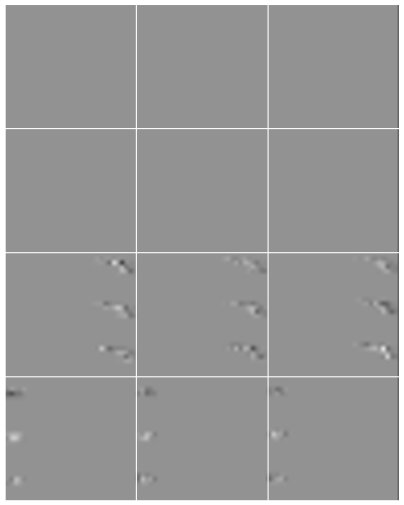
\includegraphics{inputs_orig}
\caption{Sample of maximized inputs for individual filters in the first layer of convolutions using optimal network configuration taken from Bashivan et al. Activation maps were produced by feeding empty input (an image with values of 0 for each pixel) to the network. Inputs were then iteratively tuned using gradient ascent to find the input which maximizes the activation. Many filters appear to be mostly gray and near 0, leading to the conclusion that these filters had effectively not learned anything. A similar problem was encountered in every convolutional layer.}
\end{figure}
We opted to continue using the same filter size and stride, but test different configurations for the convolutional layer and filter numbers. In order to reduce the number of dead filters, we decided to first reduce the number of filters, and then to try some alternative activation functions specialized to combat the “dead filter” problem. After evaluating a number of different layer configurations, we found that using one layer of 32 filters, followed by one layer of 64 filters, and finally one layer of 128 filters produced the optimal results in terms of reconstructing the input. 
\subparagraph{Activation function}
\begin{figure}
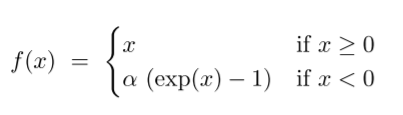
\includegraphics{elu}
\caption{ELU activation function. The exponential function for inputs below zero allows for a gradient.}
\end{figure}
As for the activation function, after consulting the relevant literature, we decided to evaluate the performance of ELUs in lieu of the ReLU activations used in the original paper. The reasoning behind this is that dead filters may be due to the fact that the gradient of ReLU for negative inputs is zero, and thus no learning can occur for these inputs. This causes filters to “die” and simply not be updated in the training phase. In contrast, the ELU has an exponential activation value for values below zero, which allows for a gradient, and thus fewer “dead” filters. After making these modifications to the convolutional autoencoder, the number of dead filters was noticeably reduced.
\begin{figure}
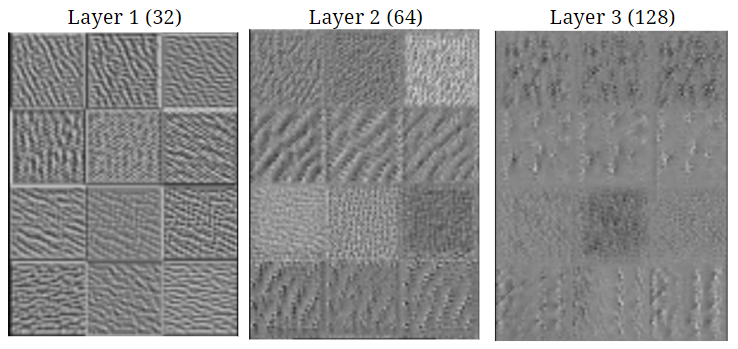
\includegraphics{inputs_optimized}
\caption{Sample of maximized inputs for individual filters after modifications. Almost every filter now appears to have learned some representation of the input.}
\end{figure}
\subparagraph{Denoising}
In an attempt to add an additional level of regularization and improve generalization, we augmented our network to add denoising. In addition to the usual benefits of denoising for neural networks, we theorized that since EEG data is inherently noisy, adding a denoising component may prove especially useful in our case. As our noise component we selected simple Gaussian noise, which was added to the inputs of the autoencoder for training, with the unmodified original image as the target output. After experimenting with the variance of the noise parameter, we found that a variance of 0.0 1 provided the best reconstruction loss on the test set, although the improvement on the test set was marginal at best. 
\begin{figure}
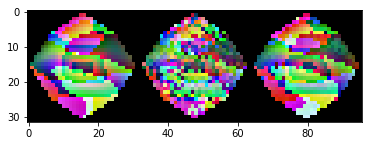
\includegraphics{denoising}
\caption{A representation of the denoising process. Left: original image; middle: input image with additional noise (variance=0.01); right: image reconstructed by autoencoder}
\end{figure}
\subparagraph{Modified cost function}
Due to the “black” areas of the image, where the EEG activation level is 0, the autoencoder is forced to learn the useless black border of the image. This wastes training time and resources. Thus a custom cost function was implemented to remove these areas from training. A mask area was identified for the border pixels, and the cost value was set to zero for these pixels. This greatly improved training speed and accuracy.
\begin{figure}
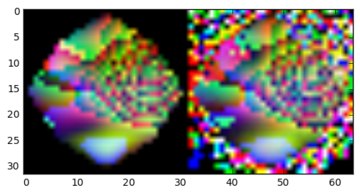
\includegraphics{mask}
\caption{Representation of output with mask (left) vs. output after training without modified cost function (right). Even after the relevant data in the image has been encoded by the autoencoder, it is still in the process of learning the black border around the image.}
\end{figure}
\subsection{Results}
\begin{center}
\begin{tabular}{ c|c|c } 
 Model & No. parameters & Accuracy \\ 
 \hline
 SVM & - & 7.78\% $\pm 4.1\% $\\ 
 Random Forest & - & 36.72\% $\pm 7.3\%$ \\ 
 Logistic Regression & - & 33.6\% $\pm 5.8\%$ \\ 
\end{tabular}
\end{center}

\section{Discussion}
Discussion content

\begin{thebibliography}{9}

	\bibitem{learning_eeg_repr} 
	Bashivan  P,  Rish  I,  Yeasin  M,  Codella  N  (2016). 
	\textit{Learning  Representations from  EEG with  Deep Recurrent-Convolutional  Neural Networks}. 
	In arXiv:1511.06448 [cs]. arXiv: 1511.06448

	\bibitem{random_forests} 
	Ho, Tin Kam (1995)
	\textit{Random Decision Forests}. 
	Proceedings of the 3rd International Conference on Document Analysis and Recognition, Montreal, QC, 14–		16 August 1995. pp. 278–282
	
\end{thebibliography}
\end{document}
